\chapter{Modelo de minería de datos}

La necesidad de comprender los procesos biológicos que están implicados en las distintas enfermedades, a partir de los datos biológicos que hay disponibles como las secuencias genómicas, los microarreglos, las interacciones proteicas, las imágenes biomédicas entre otros y la rápida adopción de las historias clínicas electrónicas proporciona una oportunidad de realizar investigaciones a gran escala. Por lo tanto las técnicas de minería de datos para el descubrimiento de conocimiento a partir de la obtención de información proveniente de diferentes fuentes son cada vez mas importantes en la investigación biológica y médica \cite{Wang2017}.\\

El mayor reto de la minería de datos genómicos esta en la extracción de información relevante de grandes volúmenes de datos clínicos y transformarlos en conocimiento, los mayores retos están en: a) La recolección de los datos clínicos y genómicos, b) recuperación de información relevante de datos y c) extracción de nuevos conocimientos de la información \cite{Farid2016}. \\  


Este capitulo esta organizado en las siguientes secciones: 5.1 Análisis exploratorio de los datos, 5.2 Análisis textual de información clínica, 5.3 Asociación de grupos con variantes, 5.4 Visualización, 5.5 Discusión y 5.6 Conclusiones y resumen. 

\section{Análisis exploratorio de los datos.}

Se realizo el análisis exploratorio de la información contenida dentro de la base de datos.Se tomo una muestra de 250 pacientes donados por el laboratorio Genetix S.A.S de los cuales solo 228 contaban con consentimiento informado para utilizar la información con fines de investigación.\\

Los datos fueron consultados desde la base de datos diseña en el cápitulo anterior y fue gestionada con la librería de python pandas \cite{mckinneypandas}. Obteniéndose los siguientes resultados:

\begin{figure}[h!]
	\centering
	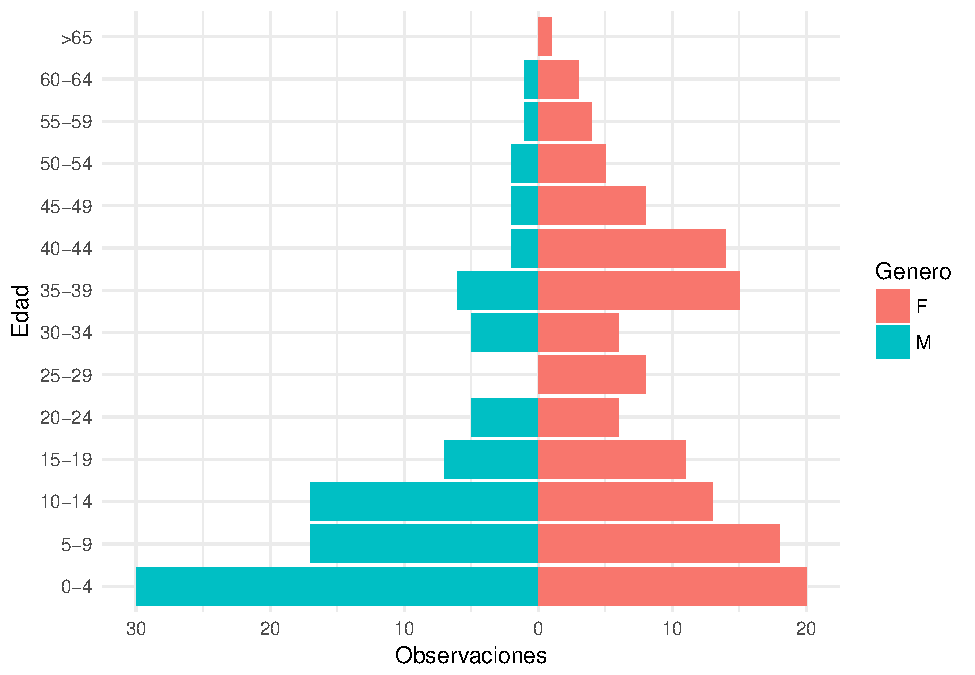
\includegraphics[width=0.5\textwidth]{Kap4/general}
	\caption{Distribución de rango de edades y géneros de los pacientes}
	\label{fig:general}
\end{figure}

\begin{figure}[H]
	\centering
	\subfigure[Distribución de variantes según su tipo.]{
		\label{f:generosgeneral}
		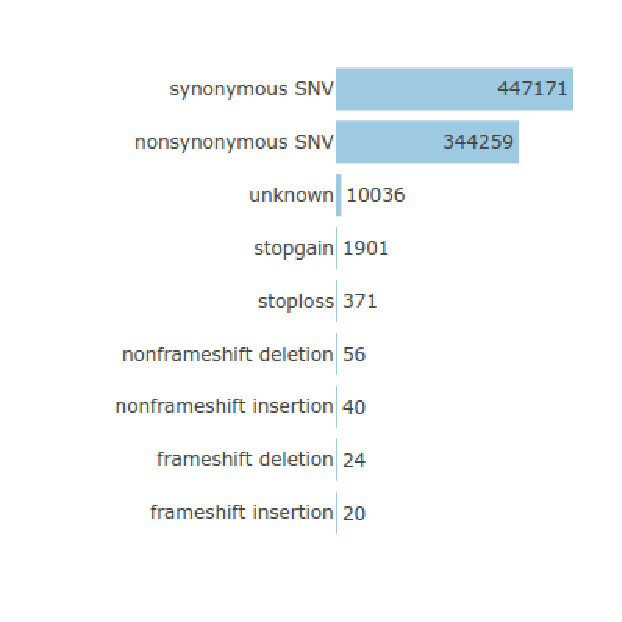
\includegraphics[width=0.35\textwidth]{Kap4/variantes.png}}
	\subfigure[Distribución de variantes por rango de edad]{
		\label{f:variantedad}
		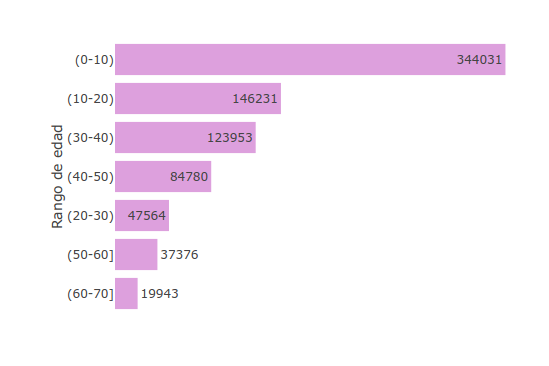
\includegraphics[width=0.55\textwidth]{Kap4/edad.png}}
	\caption{Distribución del tipo de variantes}
	\label{f:variantesgeneral}
\end{figure}

La base de datos contiene 228 pacientes de los cuales 133 son de género femenino y tienen un total de 468.485 variantes y 95 de género masculino con 345.239 de variantes obteniendo  un total de 803.878 variantes. La  figura \ref{fig:general} representa la distribución de pacientes por rango de edades y la figura \ref{f:variantesgeneral} representa la distribución de variantes según su tipo. En la figura \ref{f:generosgeneral} muestra el número de variantes que son sinónimas y no sinónimas siendo las más frecuentes en la población, a  nivel mundial se conoce que estos son lo tipos de variantes más frecuentes\cite{Fu2013}.\\

Las variantes desconocidas son el tercer tipo de variante más frecuente dado que aún existe el problema de selección del transcripto para realizar la nomenclatura adecuada de las variantes, por lo que el anotador informa que son desconocidas \cite{McCarthy2014}. La figura\ref{f:variantedad} muestra la distribución de las variantes identificadas según el rango de edad, siendo el rango con mayor número de variantes los pacientes que se encuentran entre las edades de 0 a 10 años, dado a que es la población más representada dentro de la base de datos. \\

El estado alélico de las variantes (cigocidad) que se encuentran dentro de la base de datos se dividen en heterocigotas 458639 que corresponden al 57,05\% del total de las variantes  y homocigotas 345239 que corresponden al 42,95\%. La distribución de la cigocidad de las variantes se puede explicar desde el error que se puede generar en la identificación de las variantes dado que durante el llamado  de variantes en el que es posible que una variante homocigota se catalogue como heterocigota o si durante el proceso de secuenciación se identifican erróneamente los nucleótidos \cite{Babraham2016}\cite{Pirooznia2014}. 


\section{Análisis textual de información clínica.}

 
\subsection{Preprocesamiento.}

El proceso de limpieza y nacionalización de texto se realizo de la siguiente manera:

 \begin{enumerate}
 	\item Remoción de stop words en español, tildes y caracteres especiales como  la letra ñ y todos los documentos se unificaron en letras minúsculas.
 	\item Teniendo en cuenta la información clínica se creo un diccionario de sinónimos, donde se reemplazaron palabras que hacen referencia a una misma característica.
 	\item Calculo de la frecuencias de palabras dentro de los documentos. 
 	\item Se removieron las palabras pam,pacientes, secuenciación y gen dado que no son un factor diferenciador de los documentos.  	  
 \end{enumerate}

\subsection*{Resultados}

Los resultados que se obtuvieron para la frecuencia de palabras fueron seno, cáncer, síndrome, sospecha y años. La figura \ref{fig:sin} muestra las primeras 30 palabras más frecuentes y la nube de palabras de todos los documentos.\\

\begin{figure}[]
	\centering
	\subfigure[Nube de palabras]{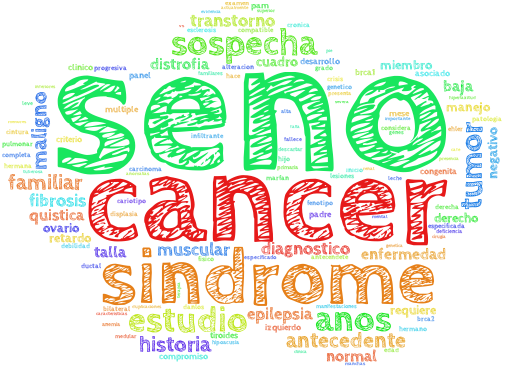
\includegraphics[width=60mm]{Kap4/sin_stop}}
	\subfigure[Frecuencia de términos]{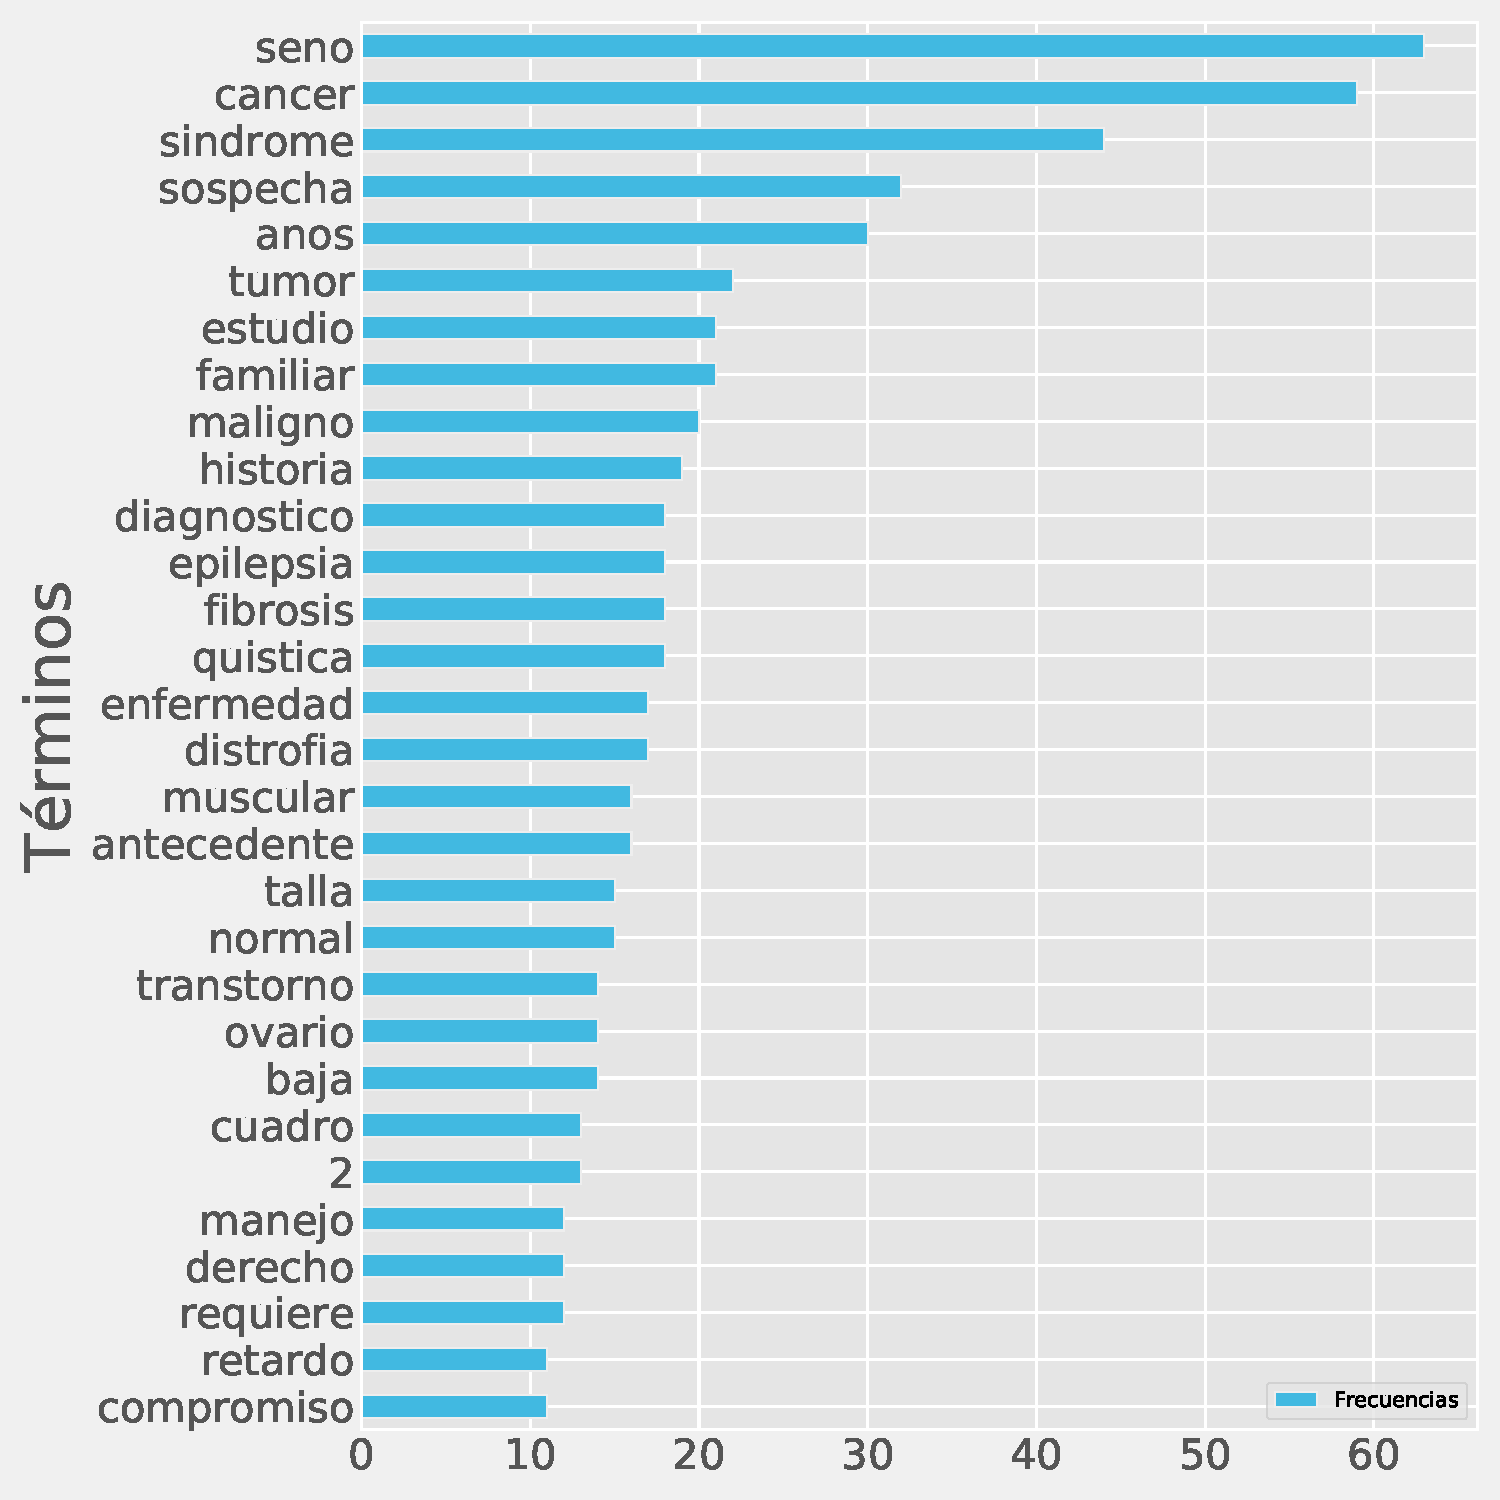
\includegraphics[width=60mm]{Kap4/frecuecias.pdf}}
	\caption{Frecuencias sin stop words y palabras sinónimas} \label{fig:sin}
\end{figure} 

Las frecuencia de palabras nos muestra las principales características de la información clínica siendo las palabras cáncer y seno los principales fenotipos, también se encuentra la palabra síndrome que puede asociarse a diferentes  enfermedades y la palabra sospecha hace referencia a diagnósticos ambiguos que pueden tener los pacientes, una de las contribuciones de la secuenciación es que basado en el fenotipo puede ayudar a un diagnóstico,entre diferentes síntomas y síndromes que pueden ser aplicados a enfermedades raras y complejas\cite{Tetreault2015a}. \\

\subsection{Grupos de características clínicas.}

En los procesos médicos, la relación entre los factores que pueden afectar la salud juega un papel importante. Una de las relaciones más comunes es la relación entre los genes y las enfermedades donde la secuenciación de exones tiene una alta aplicabilidad. Pero la identificación manual de este tipo de relaciones es compleja dada la cantidad de características que se pueden presentar como el diagnóstico propio de la enfermedad y/o la respuesta a los tratamientos \cite{Kawashima2017}.\\

La minería texto y puede ser aplicado al análisis en la medicina, donde el clustering (agrupamiento) puede ser considerado el método más importante que se utiliza en aprendizaje de maquina no supervisado que ha sido aplicado a diferentes problemas\cite{Kawashima2017}, teniendo en cuenta que no de los objetivos del agrupamiento de datos, es la  identificación de grupos naturales en datos sin etiquetas\cite{Jain2010}.\\

Partiendo de lo anterior el presente trabajo se implemento un modelo de agrupamiento utilizando el kmeans  para identificar grupos de características clínicas con la siguiente metodología:

\begin{enumerate}
	\item Cálculo de la matriz tf-idf y se normalizo. 
	\item Estimación de el número de k optimo.
	\item Implementación del algoritmo k-means.
	\item Validación de los clusters.
	\item Análisis de resultados. 	  
\end{enumerate}

\subsubsection{Transformación de los datos.}

El cálculo de la matriz tf-idf, se realiza a partir de frecuencia invertida con la ecuación 
$${idf}_i = \log_2 \frac{|D|}{|\{d \mid t_i \in d\}|}$$
siendo $|D|$ lo que denota el número total de documentos y donde $|\{d\mid t_i \in d\}|$ en  que $t_1$ aparece, la matriz de tf-idf es calculada a partir de la multiplicación de la frecuencia de términos y la frecuencia invertida $\mathit{tf}_{i,j} \cdot \mathit{idf}_i$ \cite{Buckley1988}. 
La figura \ref{fig:IDFTF} representa la matriz IDF-TF de las palabras que se encuentran dentro de la base de datos.  

\begin{figure}[H] 
	\centering
	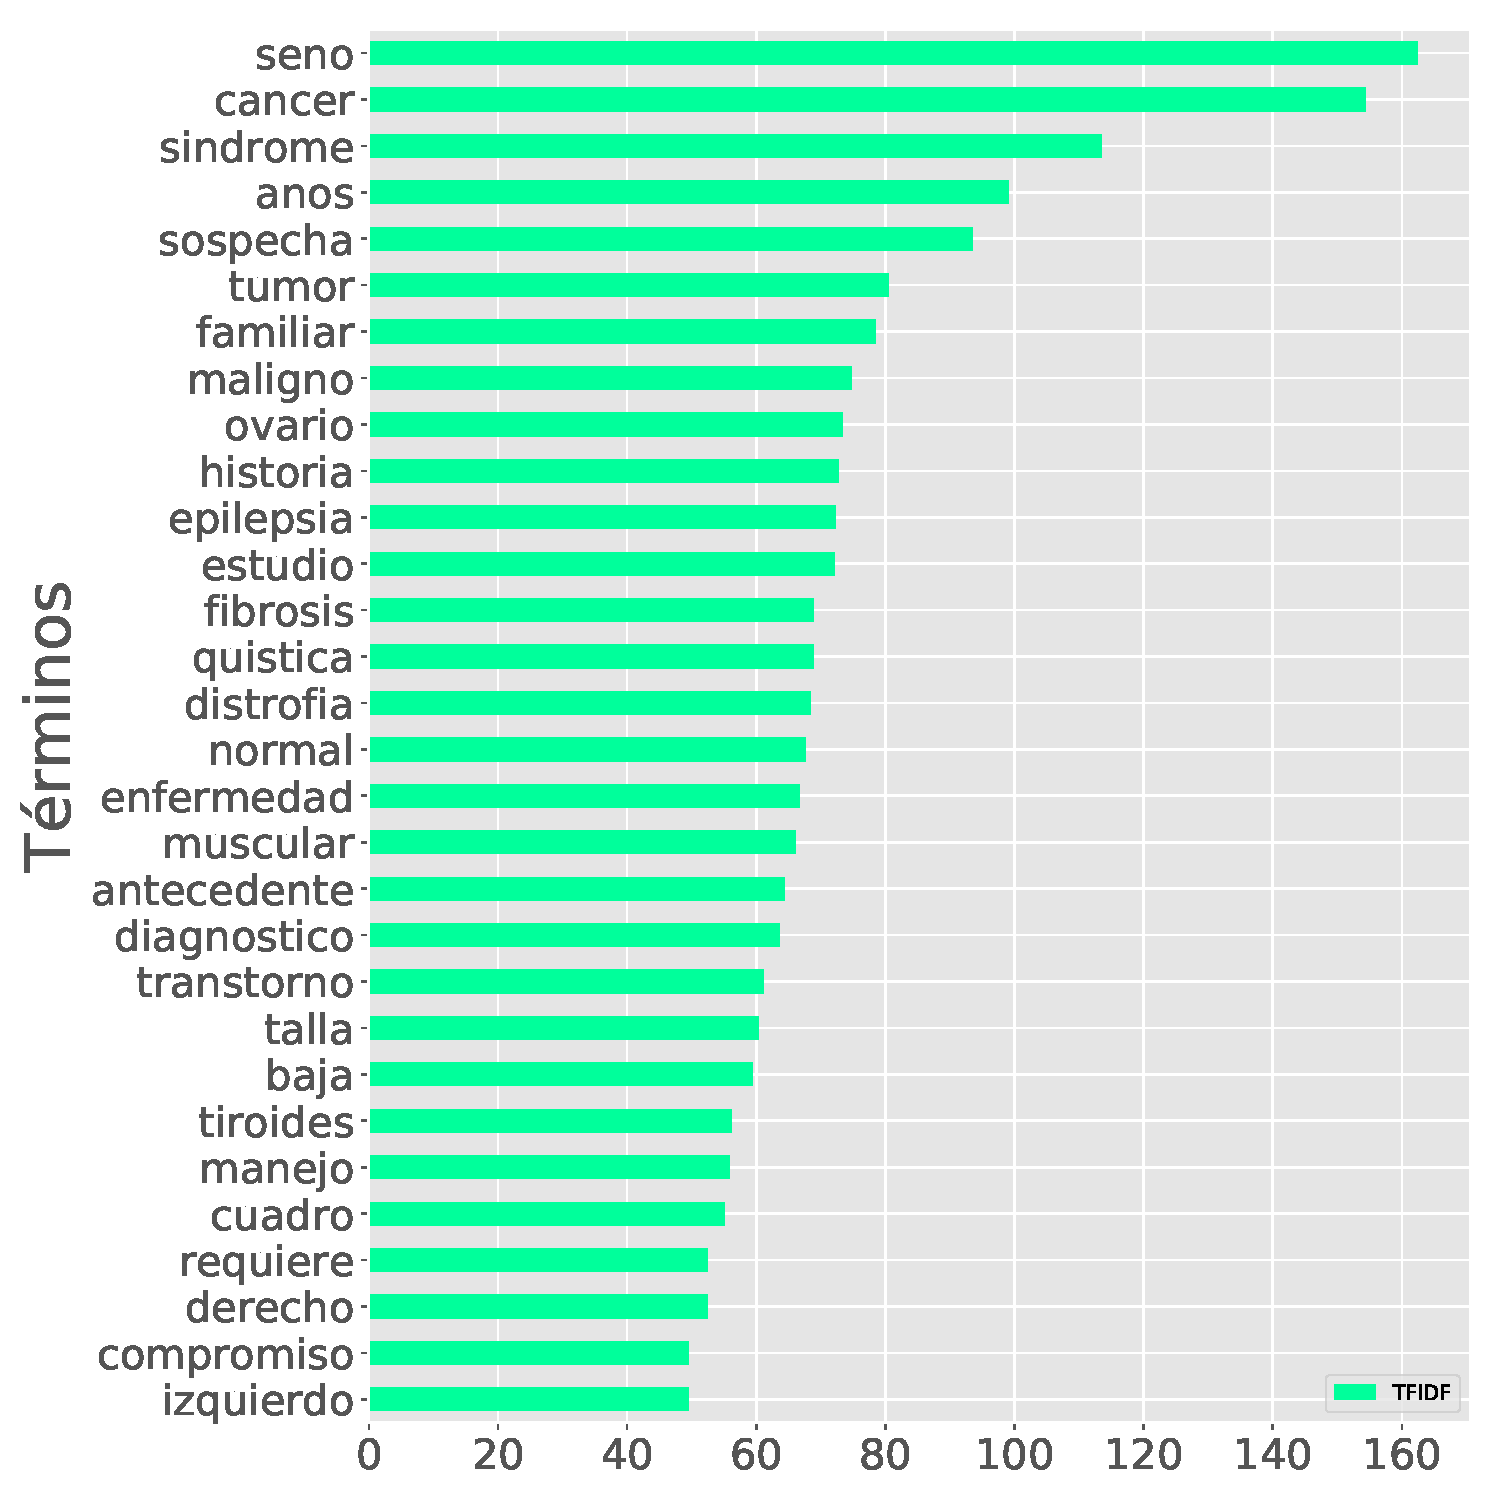
\includegraphics[width=0.5\textwidth]{Kap4/tfidf.pdf}
	\caption{TF-IDF} 
	\label{fig:IDFTF}
\end{figure}

Una vez obtenida la matriz tf-idf se normalizo y se le aplico la similaridad de coseno que es una de las medidas más populares para aplicar en documentos de texto. Esta medida tiene como ventaja que es independiente del largo del documento \cite{Huang2008}.Esta similitud fue computada de acuerdo a la siguiente formula donde la similitud ente $u$  y $v$ es definida como  según la librería scipy de python \cite{scipy}, Donde posteriormente los datos fueron utilizados para el clustering:
$$   1 - \frac{u \cdot v}
{||u||_2 ||v||_2}. $$

donde $u.v$ donde el punto es el producto de $u$ y $v$.

\subsubsection{Validación del modelo de clustering.}

La selección del número óptimo de $K$ se realizo utilizando el método del codo, este es uno de los métodos más antiguos para determinar el número de de cluster, se realizan varios experimentos iniciando por un $K$ = 2 y realizando un incremento de 1, para los cuáles se calcula el costo que conlleva cada una de las ejecuciones; entre más se aumente el número de $K7$ el costo disminuye y el número de $K$ alcanza una meseta, este valor es el que se desea obtener, visualmente se realiza la identificación mediente un gráfico de error cuadrático y número de clusters , la razón es que al continuar el aumento del número de K los nuevos clusters son muy cercanos a otros ya generados \cite{Kodinariya2013}.\\   

El cálculo del error cuadrático vs el número de clusters se realizo utilizando la libreria de python scikit learn, donde se computa el valor de la inercia que es calculada como la suma de cuadrados por cada punto cercano al centroide y es asignado al cluster. Así que  $I = \sum_{i}(d(i,cr))$ donde $cr$ es el centroide que fue asignado al cluster y $d$ es la distancia cuadrada \cite{scikit-learn}. 

\begin{figure}[H] 
	\centering
	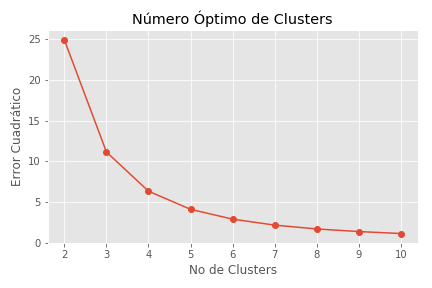
\includegraphics[width=0.5\textwidth]{Kap4/Clusters}
	\caption{Número optimo de clusters} 
	\label{fig:Clusters}
\end{figure}

Una vez se computo la inercia se realizo genero el gráfico del error cuadrático vs el número de clusters  la figura \ref{fig:Clusters} muestra el gráfico de codo obtenido, donde se puede seleccionar el cluster 5 y 6 como óptimo de $K$.\\

Para definir el número de optimo de $K$ también se computo el coeficiente de Silhouette que es una evaluación de los clusters, donde los valores altos son relacionados a modelos que tienen clusteres bien definidos .El coefiente está definido por cada muestra y está compuesta por dos valores que son \cite{scikit-learn,Rousseeuw1987}:

\begin{itemize}
	\item \textbf{a:} La distancia media entre una muestra y todos los puntos de la misma clase.
	\item \textbf{b:} La distancia media entre una muestra y todos los otros puntos en el próximo cluster más cercano.
\end{itemize}

El coeficiente Silhouette $s$ para una sola muestra se da como:

$$s = \frac{b-a}{max(a,b)}$$

Para un set de datos el coeficiente Silhouette es el promedio del coeficiente por cada muestra \cite{scikit-learn,Rousseeuw1987}. En el presente trabajo los resultados del coeficiente de Silhouette fue de  \textit{0.534}, adicionalmente se gráfico los valores de del coeficiente Silhouette para un $K$ = 5 y se presenta en la figura \ref{fig:S}:

\begin{figure}[H] 
	\centering
	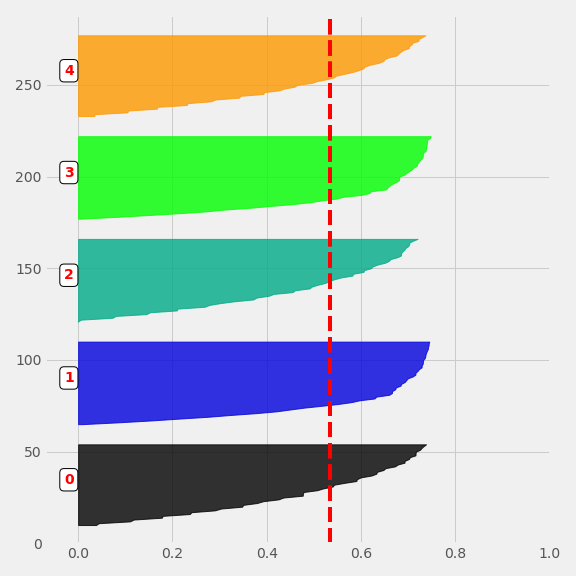
\includegraphics[width=0.3\textwidth]{Kap4/S}
	\caption{Valor Silhouette por cada cluster} 
	\label{fig:S}
\end{figure}

Para los clusters obtenidos se calcularon las medidas de validación que están dentro de la librería scikit-learn \cite{scikit-learn} son:

\begin{itemize}
	\item  \textbf{Homogeneidad:} Definida como donde cada cluster contiene solo datos de una misma clase.
	\item \textbf{Integridad:} Donde todos los miembros de una misma clase son asignados al mismo clúster.	
	\item \textbf{V-measure:} Es la medida armónica ente la homogeneidad y la integridad \cite{Rosenberg2007}. 		
\end{itemize}

El cálculo de la homogeneidad y la integridad del cluster es realizada por:
$$h=1- \frac{H(C|K)}{H(C)} $$

$$c=1- \frac{H(K|C)}{H(K)}$$

donde $H(C|K)$ es la entropía condicional de las clases en cada asignación de cluster y que son calculadas por:

$$H(C|K)= - \sum_{c=1}^{|C|} \sum_{k=1}^{|K|} \frac{n_c,_k}{n} . \log \frac{n_c,_k}{n_k}$$ 

y $H(C)$ es la entropia de clases y es calculada:
$$H(C)=  - \sum_{c=1}^{|C|} \frac{n_c}{n} . \log \frac{n_c}{n}$$ 
con $n$ que es el número total de muestras $n_c$ y $n_k$ son el número de muestras asignadas respectivamente a la clase $c$ y al cluster $k$, y finalmente $n_c,_k$ son el número de muestras de las clases$c$ asignadas al cluster $k$.

Finalmente el V-measure está definido de la siguiente manera \cite{Rosenberg2007}:

$$v= 2.\frac{h.c}{h+c}$$

También se calculo Rand-Index que calcula una medida de similitud entre dos grupos al cosiderar todos los pares de las muestras y los pares de conteo que se asignan al mismo cluster o en diferentes grupos. Calculado de la siguente manera \cite{scikit-learn}:
$$ARI = (RI - Expected_RI) / (max(RI) - Expected_RI)$$

Los resultados de validación obtenidos fueron:

Para homogeneidad 0.296, para integridad 1.0, para el V-measure 0.457 y el Rand-Index fue 0. La homogeneidad perfecta sería con un valor de 1.0, en los presentes clusters presentan una baja homogeneidad, pero una una integridad de 1.0 que significa que las etiquetas son perfectamente completas, esto se ve reflejado en el V-measure que es de 0.457 donde tenemos clusters con baja homogeneidad pero una alta integridad.  Rand-Index se obtuvo un valor de 0.0 que muestra que las clases están separadas en diferentes clusters \cite{scikit-learn}. 

\section{Asociación de grupos con variantes.}

Una vez realizado el agrupamiento de la información clínica se aplico un modelo de asociación de las variantes con los clusters obtenidos de la siguiente forma:

\begin{enumerate}
	\item Consulta de las variantes que se encontraban en cada cluster.
	\item Asociación de las variantes por cluster.
	\item Asociación de las variantes por toda la información de la base de datos filtrada por el gen CFTR como caso de ejemplo.
\end{enumerate}

La minería de datos frecuentes y las reglas de asociación  es un método popular y bien investigado par describir las relaciones entre variantes en grandes bases de datos \cite{Hahsler2005}. Las reglas de asociación (RA) muestran atributos con valores que ocurren frecuentemente en el set de datos, es posible obtener todos las posibles reglas de algunos atributos de acuerdo a la presencia de otros atributos \cite{Karabatak2009}.\\

Las reglas de asociación se basan en un set de items(elementos) $I = \{i_1,i_2,.....i_n \}$ que son un conjunto de $n$ atributos binarios. También se tiene que $D = \{t_1,t_2,..... t_m\}$ son el número de transacciones en la base de datos, cada transacción $D$ tiene una identificación única y contienen un subconjunto de elementos en $I$. Una regla se define como una implicación de la forma $X \Rightarrow Y$ donde $X,Y \subseteq I$ y $X \bigcap Y = \emptyset$. Los sets de elementos son llamados $antecedentes$ y $consecuentes$ \cite{Hahsler2005,Karabatak2009}.La selección de reglas interesantes se realiza calculando la confianza y el soporte que son definidos como:

\begin{itemize}
	\item Dados un set de datos $X \Rightarrow Y$, en una \textit{regla de asociación} tiene una confianza $c$ si $c$ de nuestra transacción que contiene $X$ pero que también contiene $Y$ \cite{Agrawal1994}.
	
	\item Dados un set de datos $X \Rightarrow Y$ tiene una \textit{regla de asociación} tiene un soporte $s$ si $s\%$ de las transacciones en nuestra base de datos de transacciones que contienen $X\cup Y$ \cite{Agrawal1994}. 
	
	\item Los algoritmos de asociación tratan de encontrar todas las reglas que tengan un mínimo de soporte y un mínimo de confianza\cite{Agrawal1994}. 

\end{itemize}

\subsection{Variantes vistas como transacciones.}

Uno de los criterios más importantes para la clasificación de variantes es la frecuencia con la que se presentan las variantes dentro de una población según la asociación americana de genética médica \cite{Laboratories2015}, otro de los retos de los análisis de variantes es el estado alélico de las variantes, que se define como una forma alternativa de un gen, en este caso se aplica a las variantes encontradas dentro de la secuenciación; existen tres tipos de estado alélico: el primero es el homocigoto donde los dos alélos son idénticos, el heterocigoto cuando los alélos son diferentes y el heterocigoto compuesto que hace referencia a dos variantes heterocigotas que afectan diferentes copias del gen o la misma copia \cite{Klug2013,Compound2012}.\\

Teniendo en cuenta lo anterior es importante visualizar el estado alélico de las variantes \cite{Hannah-Shmouni2015,Laboratories2015} ya que pueden tener un impacto el fenotipo del paciente.La identificación entre la relación genotipo-fenotipo, se ingresan como frecuencia de variación, que para el trabajo caso serían las transacciones\cite{Breuer2017}.\\

La relación genotipo-fenotipo que se observa es  la de utilizar los datos de gen, el tipo de variante, la edad, el género y el clúster (representación del fenotipo), como los patrones a recibir, para mirar las asociaciones y las reglas dentro de todo el set de datos. La identificación de patrones frecuentes, puede ser aprovechado por reglas de asociación y con ello identificar los estados alélicos de las variantes en los genes que se encuentran dentro de la base de datos \cite{breuler2017}.\\

\subsection{Experimentación}

La confianza y el soporte para este trabajo se ajusto a partir de los resultados experimentales, donde se observo que el soporte es inversamente proporcional a la confianza, esto se debe a la cantidad de variantes que se encuentran dentro de la base de datos. Al correr un experimento con soporte de 0.2 y una confianza de 0.9 no se generaban ningún tipo de regla, por lo tanto se fue disminuyendo en 0.1 el valor de la confianza y el soporte, finalmente se ajusto un soporte de 0.05 y una confianza de 0.6, dado que con un soporte de 0.1 solo se generaban 5 reglas, utilizando toda los datos disponibles. Una vez realizado este ajuste se dejaron los valores de soporte y confianza igual para todos los experimentos.\\

Una vez se ajustaron los valores de soporte y confianza se realizaron 12 experimentos, los primeros 5 experimentos con todas las variante dentro del set de datos junto a su clusters, otro a todo el conjunto de datos aplicado con los datos y filtrado por el gen CFTR. Se volvieron a repetir los mismos experimentos pero removiendo las variantes sinónimas que son las más frecuentes dentro del conjunto de datos.


\subsection{Resultados} 

Teniendo en cuenta las medidas de validación encontramos  5 clusters con las siguientes estructuras:

\subsubsection*{Cluster 1}

\begin{figure}[H]
	\centering
	\subfigure[Nube de palabras]{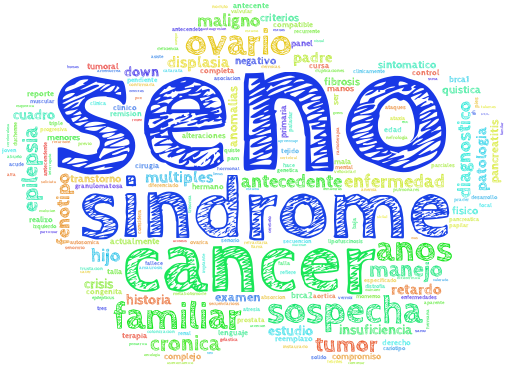
\includegraphics[width=70mm]{Kap4/cluster1}}
	\label{f:nube1}
	\subfigure[Distribucón demográfica de los pacientes]{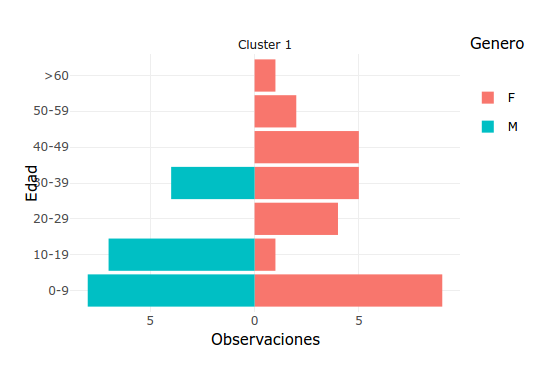
\includegraphics[width=70mm]{Kap4/edadc1}}
	\caption{Cluster 1} \label{fig:cluster1}
\end{figure} 

La figura \ref{fig:cluster1} representa el clúster 1 con la frecuencia de palabras que se agruparon para este clúster  la figura \ref{fig:cluster1}(a) se muestra la frecuencia de palabras, siendo seno,síndrome y cáncer son las palabras más frecuentes, junto con ovario,familiar sospecha y epilepsia. La figura \ref{fig:cluster1} representa la distribución de pacientes por edad y genero dentro del grupo por rango de edad en un intervalo de 10 años.\\

\begin{figure}[H]
	\centering
	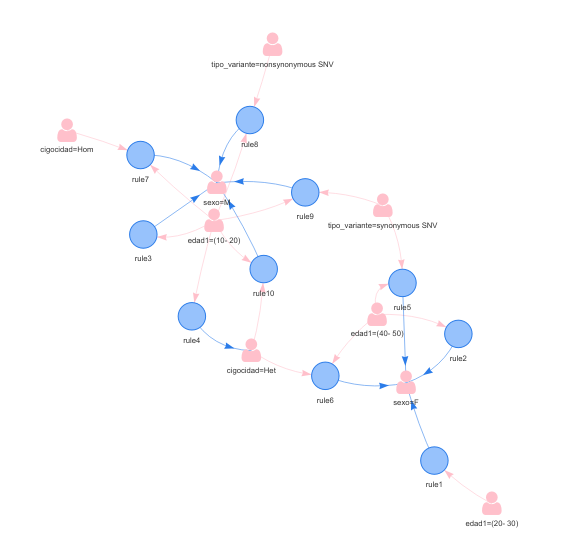
\includegraphics[width=0.8\textwidth]{Kap4/reglas1_1}
	\caption{Reglas de asociación del cluster 1 con variantes sinónimas.} \label{fig:reglas1}
\end{figure}

Las primeras 10 reglas obtenidas se representan mediante la figura \ref{fig:reglas1} que muestra la asociación,sin remover las variantes sinónimas, el resultado obtenido muestra de dos tipos de variantes dentro del clúster 1. Para el genero masculino con variantes   no sinónima y que son pacientes de edad entre 10 y 20 años, el estado alélico de las variantes es homocigoto, para este grupo se observa una alta diferencia en las reglas ambos géneros, donde las pacientes de genero femenino tienen variantes sinónimas con estado heterocigotas.

\begin{figure}[H]
	\centering
	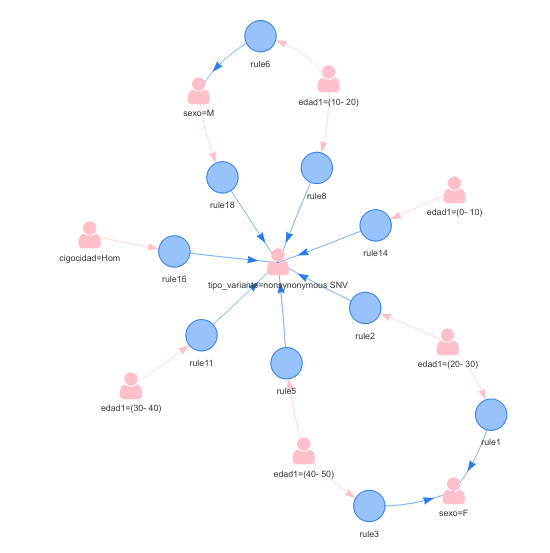
\includegraphics[width=0.8\textwidth]{Kap4/reglas1_2}
	\caption{Reglas de asociación del cluster 1 sin variantes sinónimas.} \label{fig:reglas2}
\end{figure}

Las 10 primeras reglas removiendo las variantes sinónimas que se muestran en la figura  \ref{fig:reglas2}, nos muestra nuevamente la distribución de este tipo de variante dentro del grupo, donde los pacientes masculinos son pacientes entre 10 y 20 años, con variantes heterocigotas no sinónimas, mientras que para el genero femenino se tienen rangos de edad más amplios desde la edad  de 0 a 50 años.

\subsubsection*{Cluster 2}

\begin{figure}[H]
	\centering
	\subfigure[Nube de palabras]{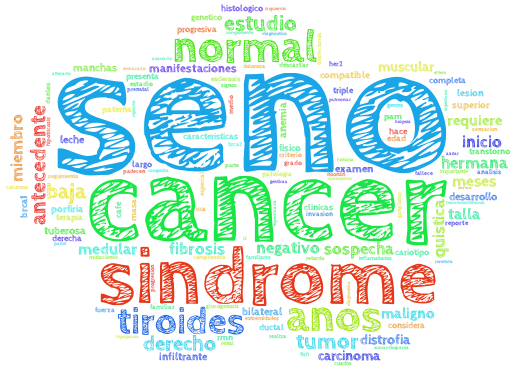
\includegraphics[width=60mm]{Kap4/cluster2}}
	\subfigure[Rango de edad en décadas.]{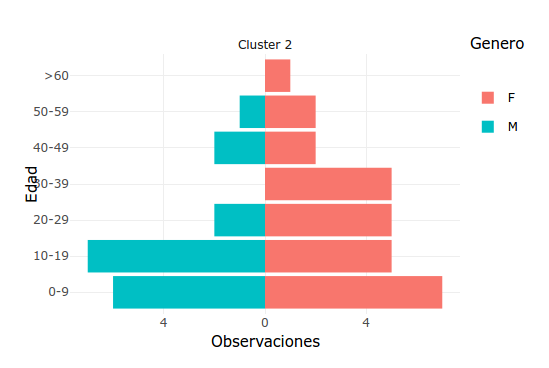
\includegraphics[width=60mm]{Kap4/edadc2}}
	\caption{Cluster 2} \label{fig:c2}
\end{figure}

En la figura \ref{fig:c2}(a) se observa que al igual que el cluster 1 las palabras más frecuentes son cáncer,seno y síndrome, pero aparecen palabras como antecedente tiroides y hermana,según la \ref{fig:c2}(b) se observa que rangos de edad entre 20 y 30 años, y mayores de 40 no hay pacientes masculinos, siendo este un cluster representado principalmente por pacientes femeninas.  

\begin{figure}[H]
	\centering
	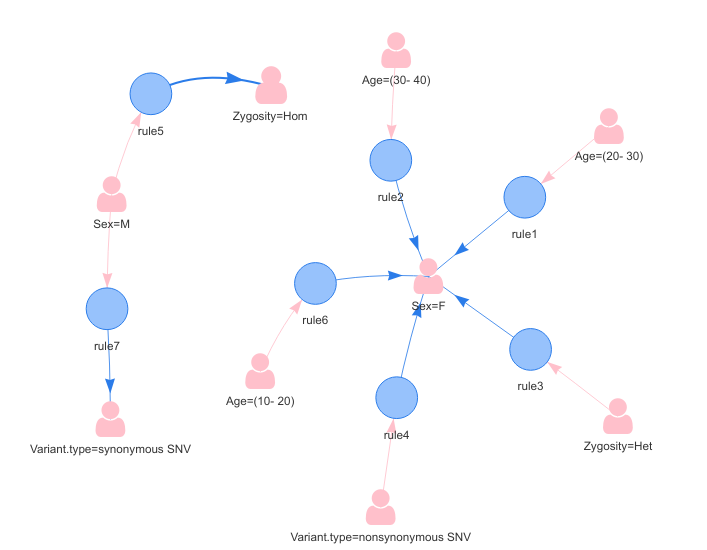
\includegraphics[width=0.8\textwidth]{Kap4/reglas2_1}
	\caption{Reglas de asociación del cluster 2 con variantes sinónimas.} \label{fig:reglas2_1}
\end{figure}

La figura \ref{fig:reglas2_1}, nos muestra unicamente una asociación de variantes al género femenino, que corresponde con la baja representación de pacientes de género  masculino.La distribución del estado alélico homocigoto se presenta en mayor frecuencia con pacientes en edad de 30 y 40 años, y son variantes de tipo no sinónimo, a pesar de que el rango de edad no es el más representativo del cluster es el que presenta una mayor frecuencia de variantes.
 
\begin{figure}[H]
	\centering
	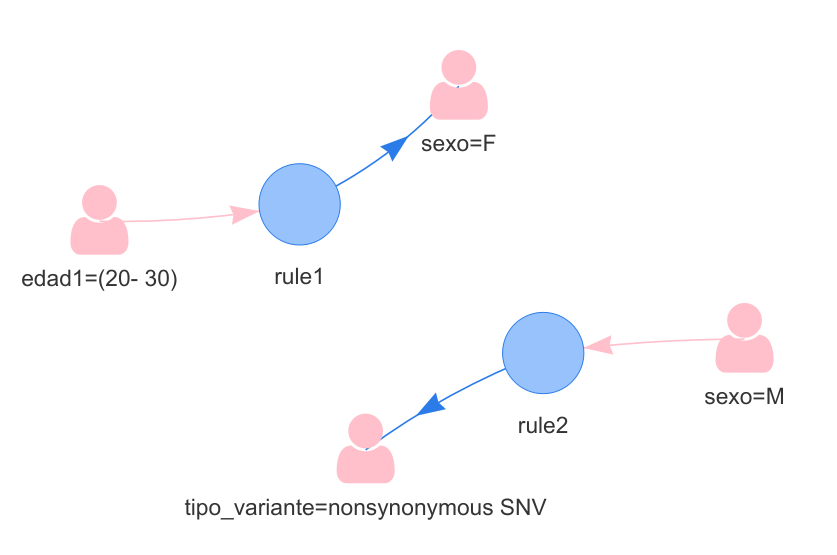
\includegraphics[width=0.8\textwidth]{Kap4/reglas2_2}
	\caption{Reglas de asociación del cluster 2 con variantes sinónimas.} \label{fig:reglas2_2}
\end{figure}

La figura \ref{fig:reglas2_2}, nos muestra la distribución de las variantes según los rangos de edad y que el tipo de variante no sinónimas, no muestra reglas para el estado alélico de las variantes dentro del clúster, solo las asociaciones entre rangos de edad y genero. 

\subsubsection*{Cluster 3}

\begin{figure}[h]
	\centering
	\subfigure[Nube de palabras.]{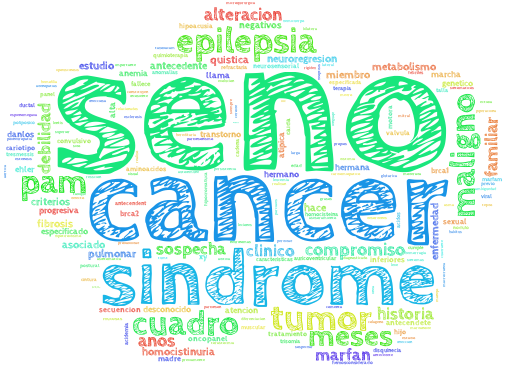
\includegraphics[width=60mm]{Kap4/cluster3}}
	\subfigure[Rango de edad en décadas.]{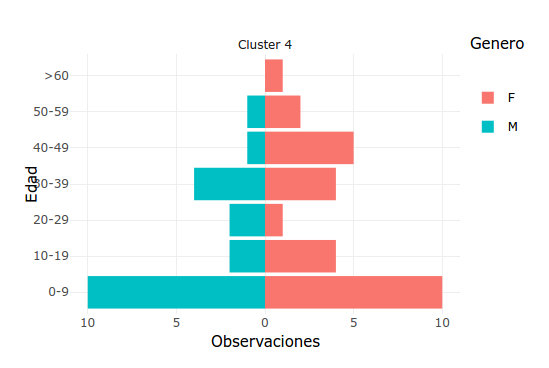
\includegraphics[width=60mm]{Kap4/edadc3}}
	\caption{Cluster 3} \label{fig:c3}
\end{figure}

La figura \ref{fig:c3}(a) nos muestra la frecuencia de palabras donde seno, cáncer y síndrome se tiene la palabra pam tumor maligno y epilepsia. La figura \ref{fig:c3}(b) muestra la distribución donde no hay pacientes de genero masculino para mayores de 60 años.  

\begin{figure}[H]
	\centering
	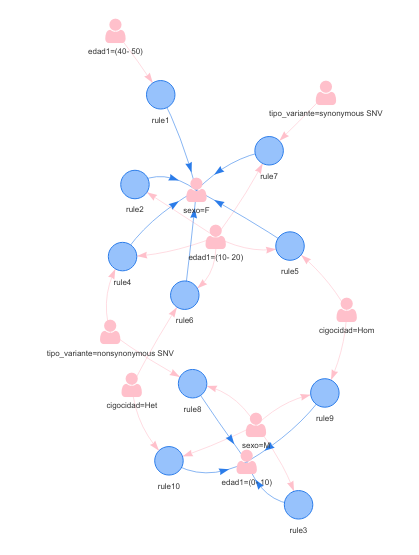
\includegraphics[width=0.8\textwidth]{Kap4/reglas3_1}
	\caption{Reglas de asociación del cluster 3 con variantes sinónimas.} \label{fig:r3}
\end{figure}

La figura \ref{fig:r3} muestra las asociaciones entre las variantes sinónimas al género femenino, donde las variantes sinónimas se encuentran en mayor frecuencia a el rango de edad entre 40 a 50 años y son heterocigotas, se presenta una frecuencia de pacientes entre los 10 y 20 años a variantes con un estado alélico homocigoto y al genero femenino, mientras que para el rango de edad de 0 a 10 años el estado alélico esta dividido entre homocigoto y heterocigoto, pero con variantes no sinónimas.

\begin{figure}[H]
	\centering
	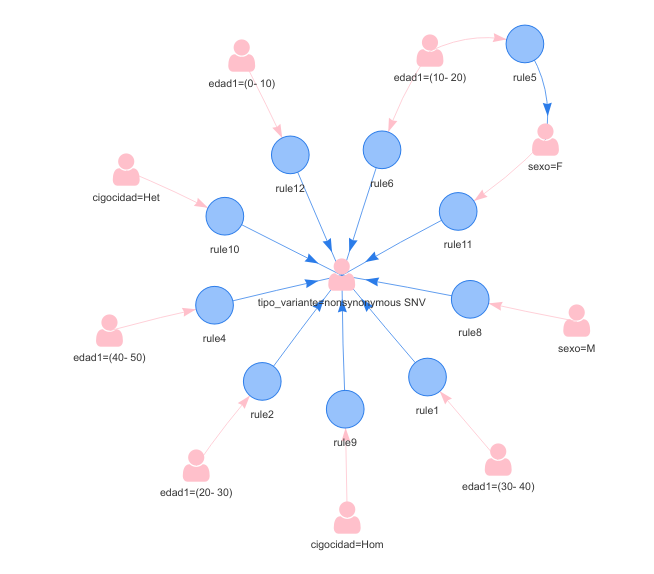
\includegraphics[width=0.8\textwidth]{Kap4/reglas3_2}
	\caption{Reglas de asociación del cluster 3 sin variantes sinónimas.} \label{fig:re3}
\end{figure}

La figura \ref{fig:re3} muestra la asociación de rangos de edades con las variantes no sinónimas donde las variantes del género masculino son para un rango de edad entre 0 y 10 años de edad, mientras que los demás rangos pertenecen no está asociados a un género en especifico, para el genero femenino se observa que el rango de edad es de 10 a 20 y de 40 a 50,mientras que los demás rangos de edad no muestran otro tipo de asociación para este tipo de variantes.  

\subsubsection*{Cluster 4}
\begin{figure}[H]
	\centering
	\subfigure[Nube de palabras]{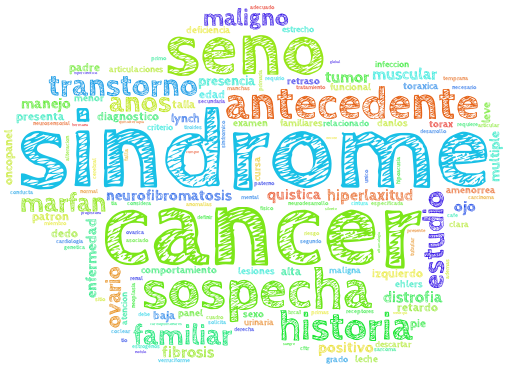
\includegraphics[width=60mm]{Kap4/cluster4}}
	\subfigure[Rango de edad en decadas]{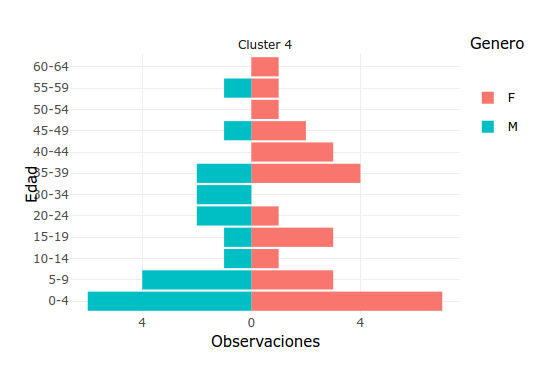
\includegraphics[width=60mm]{Kap4/edadc4}}
	\caption{Cluster 4} \label{fig:c4}
\end{figure}

La figura \ref{fig:c4}(a) muestra las frecuencias de palabras que son síndrome y cáncer, pero la palabra seno no es tan predominante como los clusters anteriores, se tienen otras palabras como sospecha, antecedente, historia y trastorno. La figura \ref{fig:c4}(b) muestra que la para este cluster los rangos de edad de 40 a 45 años, de 50 a 55 años y mayores de 60 no cuentan con representación de pacientes de género femenino.

\begin{figure}[H]
	\centering
	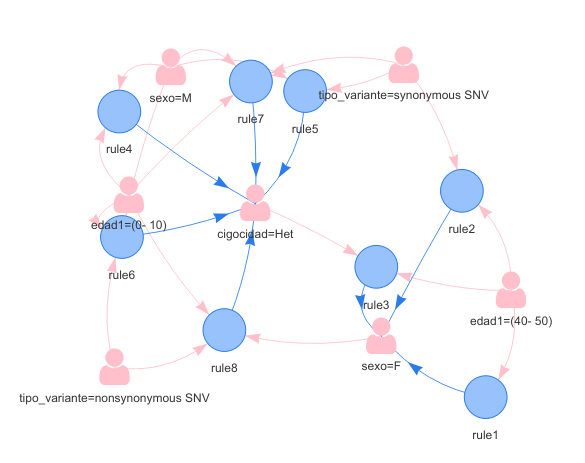
\includegraphics[width=0.8\textwidth]{Kap4/reglas4_1}
	\caption{Reglas de asociación del cluster 4 con variantes sinónimas.} \label{fig:r4}
\end{figure}

La figura \ref{fig:r4} muestra la asociación de las variante heterocigotas a pacientes masculinos de tipo no sinónimas con un rango de edad de 0 a 10 años, mientras que las variantes sinónimas se asocian a pacientes con un rango de edad de 40 a 50 años y son pacientes femeninas. 

\begin{figure}[H]
	\centering
	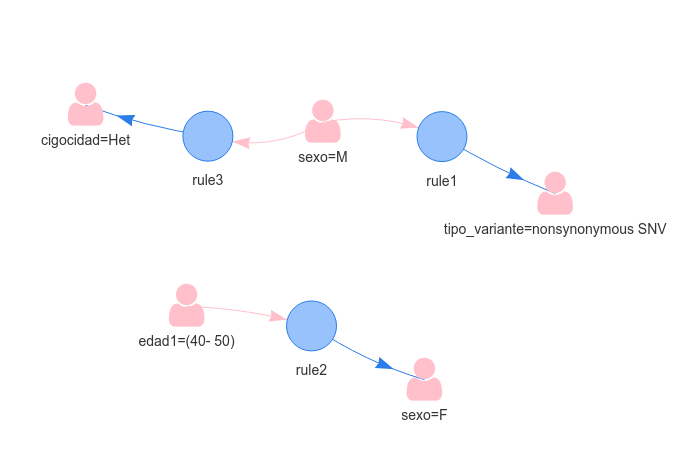
\includegraphics[width=0.8\textwidth]{Kap4/reglas4_2}
	\caption{Reglas de asociación del cluster 4 sin variantes sinónimas.} \label{fig:re4}
\end{figure}

La figura \ref{fig:re4} muestra reglas  donde las reglas del cluster nuevamente se discrimina que las variantes no sinónimas son femeninas y están en un rango de edad de (40-50), mientras que las variantes heterocigotas se encuentran en un rango de edad de 0 a 10 años. 

\subsubsection*{Cluster 5}

\begin{figure}[H]
	\centering
	\subfigure[Nube de palabras]{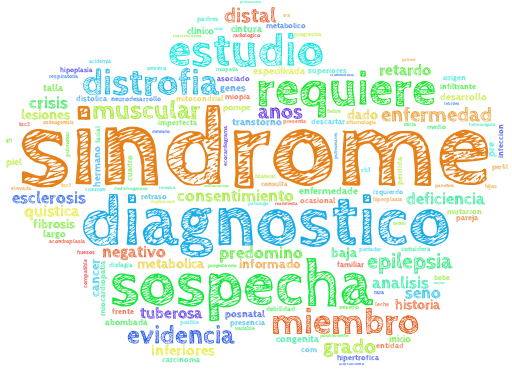
\includegraphics[width=60mm]{Kap4/cluster5}}
	\subfigure[Rango de edad en décadas]{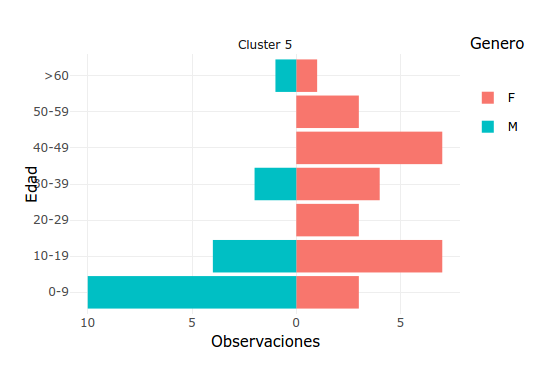
\includegraphics[width=60mm]{Kap4/edadc5}}
	\caption{Cluster 5} \label{fig:c5}
\end{figure}

La figura \ref{fig:c5}(a) presenta la frecuencia de palabras y este cluster a diferencia de todos los anteriores no presenta la palabras cáncer y seno, como las más frecuentes pero si presenta con más alta frecuencia son síndrome, diagnóstico, estudio, distrofia, requiere y miembro. La figura \ref{fig:c5}(b) muestra la distribución de pacientes por edad y género donde los rangos de 20 a 30 y 40 a 60 no se encuentran pacientes de género masculino, aunque tiene 10 pacientes masculinos en el rango de edad de 0 a 10 años.

\begin{figure}[H]
	\centering
	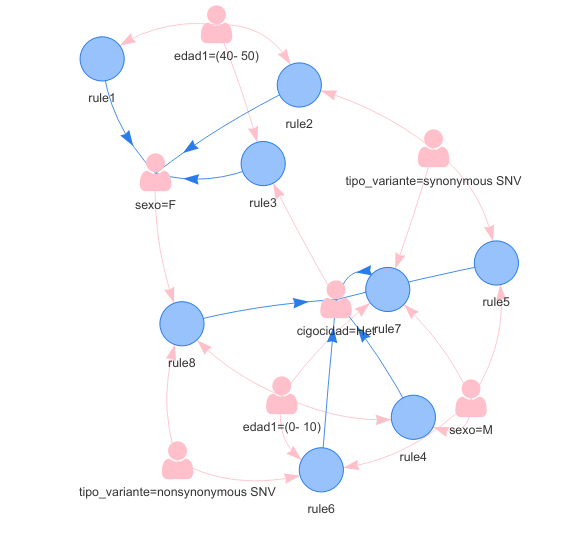
\includegraphics[width=0.8\textwidth]{Kap4/reglas5_1}
	\caption{Reglas de asociación del cluster 5 con variantes sinónimas} \label{fig:r5}
\end{figure}

La figura \ref{fig:r5} muestra la asociación de las variantes al genero femenino con un rango de edad de 40 a 50 años y de tipo sinónimas, mientras que las de género masculino  a un rango de edad de 0 a 10 años con variantes no sinónimas.

\begin{figure}[H]
	\centering
	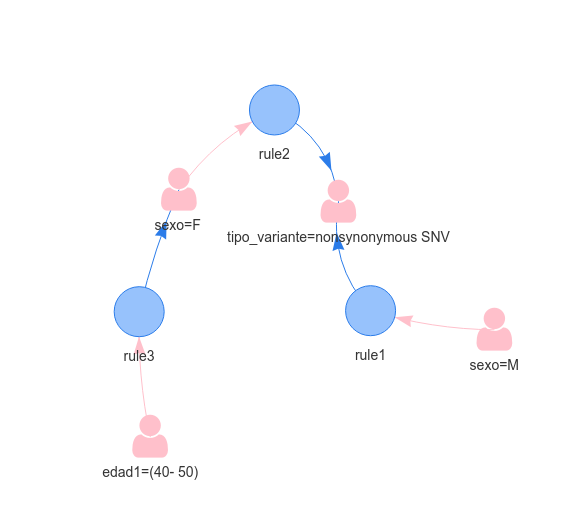
\includegraphics[width=0.7\textwidth]{Kap4/reglas5_2}
	\caption{Reglas de asociación del cluster 5 sin variantes sinónimas} \label{fig:re5}
\end{figure}

La figura \ref{fig:re5} presenta que las variante no sinónimas son más frecuentes en los pacientes con un rando de edad de 0 a 10 años y que las variantes no sinónimas presentan la regla que las variantes se encuentran en un rango de 0 a 50 años de edad son de pacientes femeninas. 


\subsubsection*{CFTR}

Visualización de reglas de asociación para toda la base de datos utilizando el gen CFTR como filtro. 

\begin{figure}[H]
	\centering
	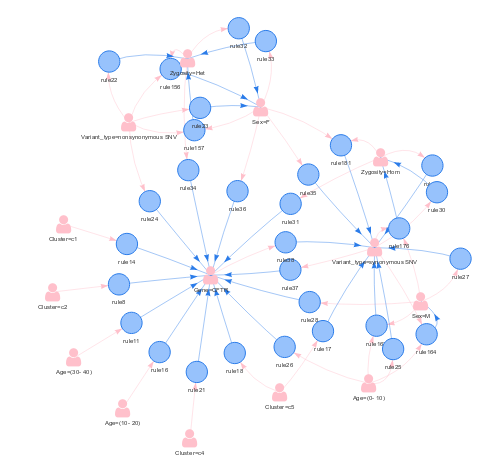
\includegraphics[width=0.87\textwidth]{Kap4/CFTR1}
	\caption{Reglas de asociación con variantes sinónimas} \label{fig:r6}
\end{figure}

La figura \ref{fig:r6} muestra las reglas 30 primeras reglas filtradas por el soporte con para toda la base de datos utilizando parámetro el gen CFTR, donde se observa que las variantes homocigotas son de tipo sinónimas y están más representadas en pacientes de ambos géneros, también se denota una frecuencia en pacientes que tienen entre 0 y 10 años de edad con variantes en este gen son de género masculino. \\

Las pacientes femeninas se tiene el caso de que las variantes son no sinonimas y no hay un  rango de edad directamente asociado a las pacientes femeninas. Los rangos de edad de 10 a 20 y de 30 a 40 tienen una frecuencia de variantes para el gen CFTR igual o mayor al 60\%, lo mismo se presenta con cluster 1,2 y 4. Para cluster 5 si se presenta una alta frecuencia de variantes sinónimas, mientras que para el cluster 3 no aparecen reglas con alta frecuencia con variantes en el gen CFTR. 

\begin{figure}[H]
	\centering
	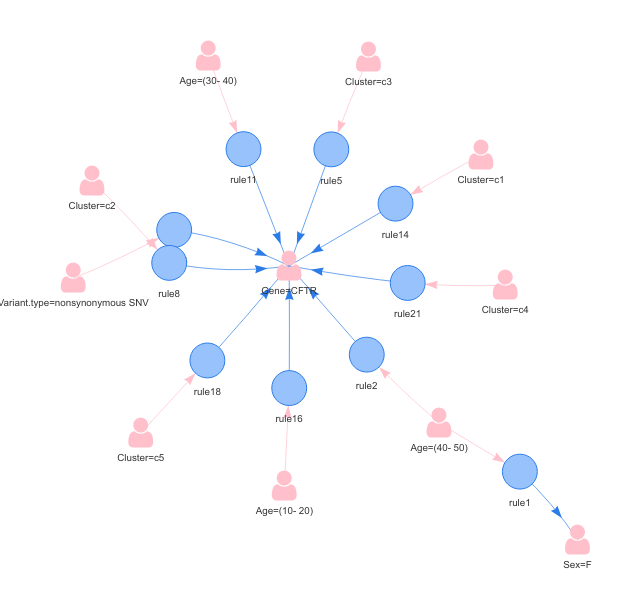
\includegraphics[width=0.8\textwidth]{Kap4/CFTR2}
	\caption{Reglas de asociación sin variantes sinónimas} \label{fig:re6}
\end{figure}

La figura \ref{fig:re6} muestra que el estado alélico de las variantes que no son sinónimas, y el estado alélico es heterocigoto para ambos generos, pero el rango de edad entre 0 y 10 años es frecuente para este tipo de variantes,a diferencia de la figura \label{fig:r6} solo se observa una alta frecuencia de las variantes no sinónimas al gen CFTR en cluster 4.  

\section{Visualización}

Finalmente se desarrollo un dashboard utilizando la herramienta R, para mostrar todos los resultados obtenidas en el presente trabajo, para que las variantes que fueron encontradas puedan ser consultadas por la comunidad académica y científica. Este aplicativo presenta una pestaña general que muestra, la distribución demográfica de la población, la distribución del tipo de variantes encontradas y la distribución de las variantes encontradas por rangos de edad. Posteriormente se muestra una pestaña con cada cluster, donde se muestran las reglas de asociación obtenidas, la frecuencia de palabras del cluster y los rangos de edad por genero del cluster. Finalmente se muestra las reglas de asociación para el gen CFTR sin las variantes sinónimas y una tabla final con las variantes anotadas se obtuvieron. La figura \ref{fig:dash} muestra un screenshot  del aplicativo de visualización desarrollado, en la que se muestra los analisis exploratorios de las variantes.

\begin{figure}[H]
	\centering
	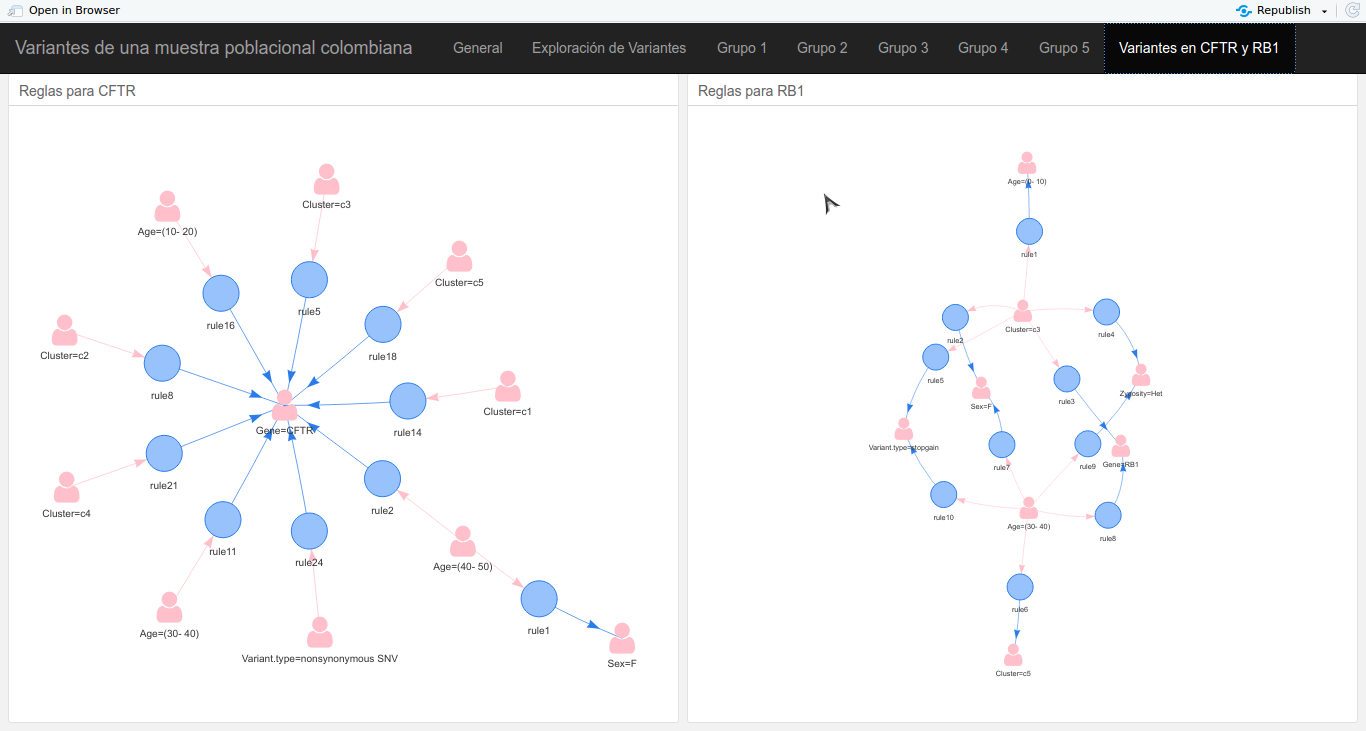
\includegraphics[width=1\textwidth]{Kap4/dash}
	\caption{Screenshot del dashboard desarrollado} \label{fig:dash}
\end{figure}

\section{Discusión}

El presente trabajo presenta los resultados de las variantes de la muestra poblacional que es de 228 pacientes y se cuenta con información como edad y genero,además que son pertenecientes a diferentes regiones del país (las muestras fueron remitidas de diferentes instituciones a nivel nacional, las muestras no contaban con la ubicación geográfica del paciente), esto en comparación con el proyecto de 1000 genomas, donde se secuenciaron 136 individuos de la ciudad de Medellín-Antioquia y el cual es un set de datos que no representan la población colombiana que es altamente diversa \cite{GabrielBedoya,Consortium2012}. Los datos que se encuentran dentro de este proyecto son utilizados principalmente para realizar análisis de ancestria \cite{Rishishwar2015a} y no evaluación de variantes dentro de la población, que igualmente no reflejan la ancestria y mezcla de la población colombiana. 

\subsection{Asociación de variantes con sus grupos de características clínicas.}

Los resultados de los grupos reflejan las características clínicas que se encuentran dentro de la base de datos, siendo el cáncer de seno el principal casual para llevar acabo las pruebas de secuenciación, esto corresponde con una de las bases para realizar la prueba de secuenciación en Colombia, ya que su valor diagnóstico y pronostico ha sido ampliamente estudiado en el país donde se da la importancia de la evaluación de la frecuencia de variantes en los genes BRCA1 y BRCA2 dentro de nuestra población, esto explica la razón de la alta frecuencia de las palabras cáncer y seno en cuatro de los cinco clusters obtenidos \cite{Ignacio2017,Arias-blanco2015}.\\

Los pacientes que se encuentran entre 0 y 10 años son la población más alta dentro de la base de datos (96 individuos)  y los que más variantes tienen, a pesar de ello las variantes que se presentan en este grupo poblacional no presentan la mismas reglas de asociación en los grupos frecuencia por ejemplo en el cluster 2 con las variantes \ref{fig:reglas2_1} se observa que no hay reglas frecuentes.\\ 

Los 4 primeros clusters están siendo representados por palabras similares, en el cuarto cluster la frecuencia de la palabra seno disminuye en comparación con los otros tres, se muestran diferencias significativas entre los rangos de edad y la distribución de géneros en cada uno de los clusters, y al incluir las reglas de asociación de cada uno de los clusters se tiene que las variantes no son iguales, inclusive a pesar de que la representación de pacientes femeninas aún es más alta la distribución de sus variantes difiere entre clusters, a pesar de que la homogeneidad de los mismos es baja, la diferencia entre cluters la composición de variantes y pacientes es altamente notoria.\\  

El cluster 5 que es único cluster las palabras cáncer y seno como las palabras más frecuentes, pero si la palabra síndrome que es común en todos los clústers, al hacer una evaluación de los pacientes, en este grupo se tienen otras palabras por lo tanto son pacientes que vienen por otras causas distintas a cáncer de seno, también es un grupo con una representación más alta de hombres. Este cluster atípico tiene una regla donde se muestra que las variantes heterocigotas no sinonimas se encuentran  en pacientes de 0 a 10 años. El hecho de que este grupo no asocie su variantes a un genero y si a un estado alélico nos puede llegar a mostrar que este grupo de pacientes tienen variantes autosomicas dominantes o variantes heterocigotas compuestas, y que las manifestaciones clínicas se presentan en una edad temprana \cite{Kamphans2013}. \\

La identificación de las causas genéticas de enfermedades por medio de la priorización de variantes partiendo de su tipo, deja una pobre aplicación de las variantes que causan perdida de la función biológica dependiendo de su estado alélico \cite{Eilbeck2017} dado que en las bases de datos normalmente el estado alélico no está disponible y su interpretación puede ser compleja \cite{Stenson2017} en el presente trabajo se muestra las variantes y su estado alélico dentro de la población muestreada. 


\subsection{Variantes con el gen CFTR}

Las variantes del gen CFTR son asociadas a la fibrosis quistica, ya que pueden ser causantes de perdida de la función biologica de la proteína, aunque la relación de las variantes con las manifestaciones no está completamente identificada, una de las razones por lo que su relación entre variante y enfermedad esta dada por la complejidad alélica de las variantes. Para este gen en particular se han reportado más de 2000 variantes pero solo unas pocas son asociadas a fibrosis quistica aproximadamente el 10\% han sido asociadas a variantes y su estado alélico. Se ha estimado que las técnicas de NGS es capaz de detectar el 80\% de las variantes del gen y tiene estimada una taza de detección de las variantes para fibrosis quistica clásica del 97\% \cite{Rowntree2003,Terlizzi2017b,Farrell2016}. El diagnostico de esta enfermedad se realiza mediante la evaluación clínica de los principales síntomas, normalmente este diagnóstico seda en los primeros años de vida \cite{Terlizzi2017b}.\\

Los rangos de edad frecuentes donde se encuentran variantes para este gen son de 0 a 20 y de 30 a 40, los demás rangos no se encuentran dentro de las reglas frecuentes, los rangos de edad de las variantes corresponden a las mismas edades en las que se realizan los diagnósticos de esta enfermedad \cite{Terlizzi2017b}, aunque el rango de 30 a 40 años de edad son pacientes adultos también ha sido referenciado y dependiendo de la etiología de la enfermedad pueden darse diagnósticos tardíos de la enfermedad para rangos de edad entre los 18 a 40 años \cite{Farrell2008}, dentro de la población estudiada no tenemos un rango de edad de 20 a 30. \\

Todos los clusters, tiene una representación de las palabras fibrosis o quistica, pero en el cluster 3 no se encuentra representado con las reglas frecuentes asociadas al gen CFTR, al realizar un filtrado de reglas para esté gen unicamente en cluster 3 tenenos que solo se generan solo 3 reglas, que asocian variantes de este gen a dos rangos de edad que son entre 50 a 60 y entre 20 a 30 unicamente al género masculino, siendo estos últimos rangos de edad tardíos para el diagnostico de la enfermedad \cite{Farrell2008}.\\

Al remover las variantes sinónimas el único cluster con alta frecuencia de variación es el clúster 4 que presenta solo 4 pacientes con cinco diagnósticos y/o sospecha de fibrosis quistica, lo que muestra que es un grupo que presenta una alta frecuencia de variantes para el gen CFTR, el estado alélico es heterocigoto para estas variaciones.\\

La evaluación de variantes en el gen CFTR y la variante no sinónima más frecuentes es CFTR:exon11:c.1408G$>$A:p.V470M que es una variante con una frecuencia poblacional a nivel mundial del 50\% \cite{Zerbino2018}, mientras que en  nuestra base de datos se encuentra en 49 pacientes del total de la muestra poblacional que corresponde al 21,49\%, por lo tanto la distribución de esta variante dentro de la población colombiana es mucho menor a la reportada a nivel mundial.\\

Teniendo en cuenta que la identificación de las variantes anotadas pueden presentar un error que depende de la selección de transcripito es una de las limitaciones para generar reglas según la anotación de la variante, además de que una misma variante puede tener múltiples anotaciones,la utilización del código rs tampoco es suficiente ya que la mayoría de las variantes no cuentan con este identificador, y en ocasiones múltiples variantes que afectan la misma posición genómica tienen un mismo identificador \cite{Liu2016,McCarthy2014}. \\  

Aunque existen pacientes con sospechas y/o diagnósticos de pacientes con fibrosis quistica encontramos que las variantes patogénicas más frecuentes dentro de la población colombiana no se han identificada \cite{Vasquez2010}, dado que las regiones de splicing han sido removidas en el presente estudio, lo que limmita la evalución de la asociación de tipos de variantes que no se encuentran en regiones codificantes de genes, y no se observan otros tipos de variantes distintos a variantes sinónimos y no sinónimas. 

\subsection{Conclusión}

La utilización de técnicas de minería de datos en el campo de la bioinformática aplicada al apoyo diagnostico y  la agrupación de pacientes según sus características diagnosticas a nivel masivo junto con las variantes obtenidas a partir de técnicas se secuenciación, permiten hacer una inferencia del estado de la población y seguimiento de datos epidemiológicos de las variantes y sus posibles efectos en fenotipos de los pacientes.

\subsection*{Resumen}

El presente capítulo muestra la aplicación de un modelo de minería para analizar datos clínicos y genómicos, donde las técnicas clásicas de  agrupamiento para identificar características clínicas de pacientes son útiles para diferenciar patrones de diagnóstico, la utilización de reglas de asociación para identificar variantes y su distribución dentro de la población, que muestran patrones desde diferentes puntos de vista.\\

El desarrollo de herramientas de visualización para mostrar los resultados del proceso de minería, generar análisis propios y posibles preguntas que aporten a la investigación, en el presente  trabajo se muestra la distribución de las variantes por estado alélico, edad y genero de los pacientes según el grupo al que pertenecen, también un caso de estudio para el gen CFTR que no muestra asociaciones patogénicas en los pacientes estudiados.




   
